\documentclass{article}

% if you need to pass options to natbib, use, e.g.:
%     \PassOptionsToPackage{numbers, compress}{natbib}
% before loading neurips_2021

% ready for submission
% \usepackage{neurips_2021}

% to compile a preprint version, e.g., for submission to arXiv, add add the
% [preprint] option:
%   \usepackage[preprint]{neurips_2021}

% to compile a camera-ready version, add the [final] option, e.g.:
\usepackage[final]{neurips_2021}

% to avoid loading the natbib package, add option nonatbib:
%   \usepackage[nonatbib]{neurips_2021}

\usepackage[utf8]{inputenc} % allow utf-8 input
\usepackage[english]{babel}
\usepackage[T1]{fontenc}    % use 8-bit T1 fonts
\usepackage{url}            % simple URL typesetting
\usepackage[colorlinks = true, urlcolor = black, citecolor = black, filecolor = black, linkcolor = black]{hyperref}
\usepackage{booktabs}       % professional-quality tables
\usepackage{amsfonts}       % blackboard math symbols
\usepackage{nicefrac}       % compact symbols for 1/2, etc.
\usepackage{microtype}      % microtypography
\usepackage{xcolor}         % colors
\usepackage{graphicx}
\usepackage{subcaption}
\usepackage{tabularx}
\usepackage{caption}
\usepackage{array}
\usepackage[cmex10]{amsmath}
\usepackage{amssymb}
\usepackage{amsthm}
\usepackage[backend=biber, sorting=none]{biblatex}
\setlength\extrarowheight{2pt}

\addbibresource{ref.bib}

\title{PetFinder.my - Pawpularity}

\author{
  Armando Fortes$^1$, David Pissarra$^2$\\
  Machine Learning Course Fall 2021\\
  Department of Computer Science and Technology\\
  Tsinghua University, Beijing, China\\
  \small \texttt{\{ferreiracardos10$^1$, pissarrad10$^2$\}@mails.tsinghua.edu.cn}\\
}

\begin{document}

\maketitle

\begin{abstract}

\textit{Pawpularity} is a metric created by \textit{PetFinder.my}, Malaysia's leading animal welfare platform, which aims to measure pet photos' popularity. Nowadays, millions of stray animals are alone on the streets or living at shelters, waiting for a new home. Therefore, by taking advantage of the data science and machine learning fields, we may be able to predict the impact of certain features in pet photos, which might help them get more attention from the population. Consequently, we would help improve their chances of being rescued and finding loving homes.

\end{abstract}

\section{Introduction}

The significant number of stray animals around the world justifies the recent effort made by humans to find better conditions for these pets. Therefore, there has emerged a necessity for building new mechanisms and methods to generate more interest from the population in giving them new homes. With the development and application of the right machine learning techniques, we may be able to design a model which, given a picture of any kind of pet, will predict how popular it would be. Accordingly, the popularity of a homeless pet's photo is directly related to the visibility that it should receive. Moreover, a popular photo will have more attention from the public and, consequently, increase the chances of this pet being adopted. Also, the model may help identify the features and patterns which will lead to a popular photo, creating the opportunity for future pictures to have a better outcome than the previous ones.
Having a first look at the Pawpularity Contest \cite{kaggle_petfinder.my_2021} and respective dataset, we can formalize it as a supervised learning problem. Regarding this contest, a large dataset is given for both training and testing purposes, which contains various picture of domestic animals. Also, attached to each image there is a set of metadata with various features and most importantly the correspondent \textit{Pawpularity}, of course the latter is only available in the training set. Although it may also be modeled by many other machine learning approaches, as we are analysing images, we are encouraged to use some computer vision techniques such as Convolutional Neural Networks (CNN) or Transformer models based on self-attention. These types of models have represented a huge breakthrough in image analysis, being the reason for our initial intuition.

\section{Related Work}

\subsection{\textit{PetFinder.my}'s Cuteness Meter}

\textit{PetFinder.my} has been developing an algorithm - \textit{Cutness Meter} \cite{petfinder.my} -  related to this contest, which rates the cutness of a pet photo with 1 to 5 stars. The current application for this algorithm helps \textit{PetFinder.my}'s users receive feeback from the photos they upload. Thus, they may be able to understand actually how attractive their photos are and which one they definitely can improve. This algorithm is still in an experimental stage, and this is one of the motivations for the establishment of this contest. Since this is a competition, the teams who create the best performing algorithms may be invited to contribute to this cause by implementing their solutions on Malaysia’s leading animal welfare platform. Therefore, this is how we can relate \textit{Pawpularity} with the \textit{Cutness Meter}.

\subsection{The evolution of Machine Learning for Computer Vision}

Convolutional Neural Networks were first introduced in the 1980s, by Yann LeCun, in an attempt to distinguish and classify handwritten digits - \textit{LeNet}. In spite of presenting a great breakthrough in image recognition, there still were some issues regarding the scaling of this method, due to its computational complexity and need for large amounts of data. Only by the year of 2012, were we able to achieve the first strong results with CNNs. Alex Krizhevsky et al. \cite{krizhevsky2012imagenet} presented an improved CNN architecture - \textit{AlexNet} - to classify the 1.2 million high-resolution images from the ImageNet challenge into the 1000 different labels. The main techniques introduced by the \textit{AlexNet} which made this possible were the use of \textit{Dropout} to prevent overfitting, the use of the \textit{ReLU} activation function, which showed improved training performance over \textit{tanh} and \textit{sigmoid}, and also having a deeper and wider architecture. Therefore, it represents an important milestone on the evolution of the computer vision field, serving as a base for the following developed CNNs. Some notable examples of successful implementations are the \textit{GoogLeNet} \cite{Szegedy_2015_CVPR}, the \textit{ResNet} \cite{He_2016_CVPR}, the \textit{DenseNet} \cite{Huang_2017_CVPR} and many others \cite{Hu_2018_CVPR, Huang_2018_CVPR, efficientnet, Li_2019_CVPR}. Moreover, state of the art results continuously keep being achieved with various new creative approaches and architectures. Accordingly, due to the success of self-attention models, such as Transformers, in natural language processing, novel works have presented self-attention techniques to overcome the limitations presented by inductive convolutional biases \cite{dosovitskiy2021image, zhu2021deformable}. One of the newly developed Transformers, able to achieve SOTA results, was the Swin-Transformer \cite{2021swin}.

\subsection{Latest State of the Art results in Image Recognition}

Since the breakthrough of \textit{AlexNet}, Convolutional Neural Networks have been the dominating model architecture for computer vision. Many new architectures have been performing even better, compared to previous techniques. Dai et al. \cite{DBLP:journals/corr/abs-2106-04803} combined both CNNs and self-attention within their model together to form a complete network, which is presented as \textit{CoAtNet}. The latest implementation of this network - \textit{CoAtNet-7} - was able to achieve 90.88\% top-1 accuracy on ImageNet, with JFT-3B Google dataset, which consists of nearly 3 billion images, annotated with a class-hierarchy of around 30k labels. Taking advantage of existing neural networks, Xie et al. \cite{DBLP:journals/corr/abs-1911-04252} were able to train an \textit{EfficientNet} model \cite{Tan2019EfficientNetRM} on labeled ImageNet images and use it as a ‘teacher’ to generate pseudo labels on JFT-300M Google dataset. Then, a ‘student’ model could be trained on a larger \textit{EfficientNet}, combining labeled and pseudo labeled images, which were inferred previously by the ‘teacher’ model on unlabeled data. This process is iterated many times and each student model should later become a teacher model. Hence, student models will be subject to noise, so that the student generalizes better than the teacher. This self-training method was able to reach 88.4\% currently top-13 accuracy on ImageNet. Also, Xie et al. \cite{DBLP:journals/corr/abs-2003-10580} created another method – \textit{Meta Pseudo Labels} - based on the previous one. However, unlike the last self-training method where the teacher is fixed, the teacher in \textit{Meta Pseudo Labels} is constantly adapted by the feedback of the student’s performance on the labeled dataset. Thus, the teacher will generate better pseudo labels to teach the student. This semi-supervised learning method achieved a better accuracy compared to the last method, conquering an accuracy of 90.2\% on ImageNet.

\subsection{Image Memorability and Interestingness}

In recent years, the research community has started paying significant attention to popularity prediction in social media, which may be directed to all sorts of content such as messages, written posts, videos and images. Regarding the prediction of image popularity \cite{khosla2014what}, it has been settled that one may leverage social cues (which tends to relate to the context behind the user and the publication or the influence that the publisher may have in the social media platform), as well as the intrinsic cues of the image (which commonly relates to the dominant colors of the image, contrast, texture, GIST \cite{Oliva2004ModelingTS} and so on). However, the content of an image can be considerably harder to extract and correlate with popularity, when compared to text-based content. Therefore, there has been an increasing interest in analyzing various semantic attributes of images, such as image interestingness \cite{m.2013the} or image memorability \cite{p.2011what, khosla2015understanding}. Context has once again been regarded as an aspect which largely contributes to these matters \cite{m.2013the}. Moreover, with strong context, unusualness is the most important cue for interestingness. However, although it becomes more difficult to capture with weak contexts, there has also been evidence that there is a large degree of consistency among different viewers, and that some images are more interesting and memorable than others, even when there is no context or familiar elements (for example, famous monuments) \cite{p.2011what}. Here, general preferences seem to take the main role. Furthermore, image quality and  aesthetics \cite{5995467} or relative spatial features \cite{kim2013relative} are some examples of attributes that have been recently explored in substantial detail. In terms of conclusion, by analyzing the presented semantic attributes of images, a better understanding has been developed for situations where one wants to extract the images which are more likely to be remembered by viewers from a given collection. This knowledge could be applied to selecting images for illustrations, covers, user interfaces, as well as for the promotion of stray animals for adoption, which is the main cause of this project.

\section{Method}
The main goal for our model is to predict the right \textit{Pawpularity} of a given photo. This metric called \textit{Pawpularity} is between 0 and 100, and is related to how popular a pet photo can be. Fundamentally, our model will be trained from a given dataset which is composed from more than 9000 pet photos, striving for accurate predictions.

\subsection{Data Description}
A dataset with more than 9000 pet photos is provided on this \textit{Kaggle} competition. Each photo is labeled with its \textit{Pawpularity}. In addition, photo metadata is also included in the dataset, which contains multiple extra binary features \{0, 1\} for each picture, such as:
\begin{itemize}
   \item Focus - Pet is neither too close nor far.
   \item Eyes - At least 1 eye is visible (pupil should be clear).
   \item Face - Decently clear face.
   \item Near - Pet appears on significant portion of photo.
   \item Action - A pet action is detected, for instance jumping.
   \item Accessory - Photo contains either digital or physical accessory, for example digital stickers or physical toys.
   \item Group - More than 1 pet in the photo.
   \item Collage - Digitally-retouched photo.
   \item Human - Presence of humans in the photo.
   \item Occlusion - Undesirable objects blocking part of the pet.
   \item Info - Information in the photo by adding text or labels.
   \item Blur - Blurry part of the photo, especially for the pet’s eyes and face. For blurry pictures, \textit{Eyes} feature is always set to 0.
 \end{itemize}

\subsection{Metadata Insights}
Our work was initiated in  regards of analysing the given set of metadata features in order to have a better understanding on how each of the features may or may not affect \textit{Pawpularity}. Accordingly, we plotted the \textit{Pawpularity} frequency distribution and calculated the accordant mean for the total set of samples in the training set, as seen in Figure \ref{fig:pawpularity_distribution}, and also for each value of the given metadata features, as seen in Figure \ref{fig:metadata_analysis}.\\
From Figure \ref{fig:pawpularity_distribution}, we are able to conclude that the vast majority of samples are located in the [20, 50] interval for \textit{Pawpularity}, resulting in a mean value of 38.04. This could make it more difficult to generalize our inference, as there is such a high density of samples for a specific interval of \textit{Pawpularity}. Regarding Figure \ref{fig:metadata_analysis}, it is observable that for each metadata feature there is a significant discrepancy between the number of given samples for each value. For example, there are 9638 samples where \textit{Subject Focus} has a value of $0$ (which corresponds to 97.2\% of the total number of samples) whereas only 274 samples have value 1 (resp. 2.8\%). Similar unbalanced proportions can be found across the rest of the features, which is a sign that one may find it difficult to construct generalized knowledge from the given tabular data.

\begin{figure}[h!]
    \centering
    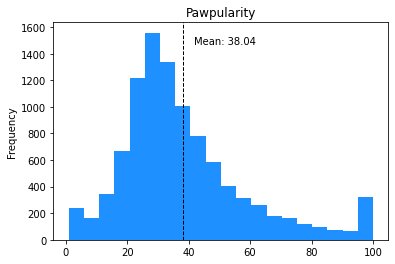
\includegraphics[width=0.65\linewidth]{figs/pawpularity_distribution.png}
    \caption{The \textit{Pawpularity} distribution for the given training set.}
    \label{fig:pawpularity_distribution}
\end{figure}
\vspace{0.5cm}

\begin{figure}[h!]
    \centering
    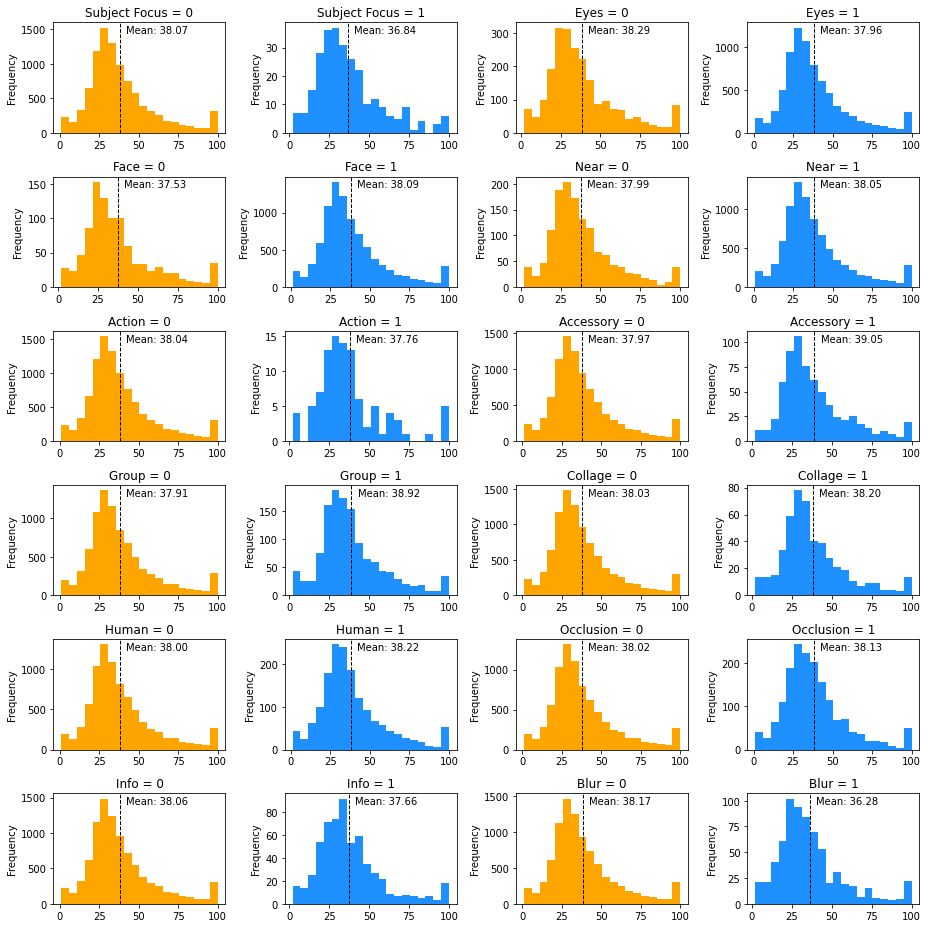
\includegraphics[width=\linewidth]{figs/metadata_analysis.png}
    \caption{The \textit{Pawpularity} distribution for each metadata feature value.}
    \label{fig:metadata_analysis}
\end{figure}

\vspace{0.3cm}Moreover, it may also be noted that all the plotted distributions in Figure \ref{fig:metadata_analysis} considerably resemble the curve seen in the plotted distribution from Figure \ref{fig:pawpularity_distribution}, as well as their identical mean values. These characteristics reiterate the hypothesis that the given metadata features may not be enough to discern whether the picture will be popular or not.\\
Furthermore, by gathering every metadata feature together, we were able to calculate the correlation between each of them and build the presented heatmap (Figure \ref{fig:correlation}).

\begin{figure}[h!]
    \centering
    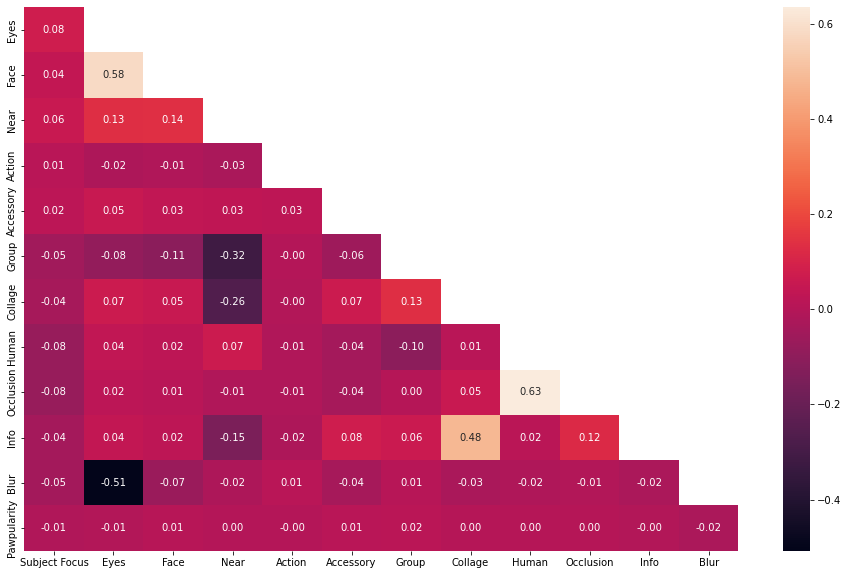
\includegraphics[width=0.8\linewidth]{figs/correlation.png}
    \caption{Correlation matrix regarding the metadata attributes.}
    \label{fig:correlation}
\end{figure}

In addition to the previous conclusions made, by analyzing the above correlation matrix between all the metadata attributes and the Pawpularity score, we understand again that there is very little connection between each feature and the desired label, which means the respective inference would have very high complexity.\\
Nevertheless, in order to further test our hypothesis, as well as potentially find combined connections between the different features, which may help extract some signals for the \textit{Pawpularity} score, we decided to use the Gradient Boosting implementation XGBoost \cite{xgboost} (Section \ref{sec:xgb}). This decision was made after several experiments with different models in an attempt to learn from the metadata features, being XGBoost the one with the best performance.

\subsection{Data Pre-Processing}
In order to build a model with improved performance, data pre-processing has an important role, since it allows the extraction of the most crucial features, as well as the removal of features and traits that can be harmful for the model, from the raw data given at the beginning.\\
Firstly, each picture is decoded into 3-Dimensional arrays of shape $W$x$H$x$C$, where $W$, $H$ and $C$ correspond to image width, image height and number of color channels, respectively. Since we will be working with Red, Green, Blue (RGB) pixel levels, there will be three channels ($C = 3$). Each entry will starts by being comprehended in [0,255] as it is the conventional interval for RGB pixel values. Subsequently, we proceed to perform normalization of our data where the resulting values are chosen to be in the range [0,1]. Data normalization is an important step where each parameter is ensured to have a similar data distribution, which has been shown to make convergence faster while training a network. Furthermore, in order to guarantee that the images have the same size, as it is required for most neural network models, each image is resized into a a square shape of dimensions 224x224, which means the final shape of the 3-Dimensional array of each picture is 224x224x3. The input will the correspond to a set of 9912 pictures the grouped into batches of size 32, where each picture is represented by the mentioned 3-D arrays. In regards of the labels, the given \textit{Pawpularity} of each picture is also normalized into a range between [0, 1], since the given dataset provide scores between [0, 100].\\
Additionally, in order to increase the size of the dataset, we implemented data augmentation. To do so, we adjusted some values, such as brightness, contrast, hue, and saturation. These augmentations were embedded inside the image batch, so the model can fetch augmentations during the learning process.

\subsection{Model Description}
The designed model for this Kaggle competition is essentially an Ensemble Model (Figure \ref{fig:arch}) from a neural network with a Swin transformer as the backbone, and a XGBoost regressor.

\begin{figure}[h!]
    \centering
    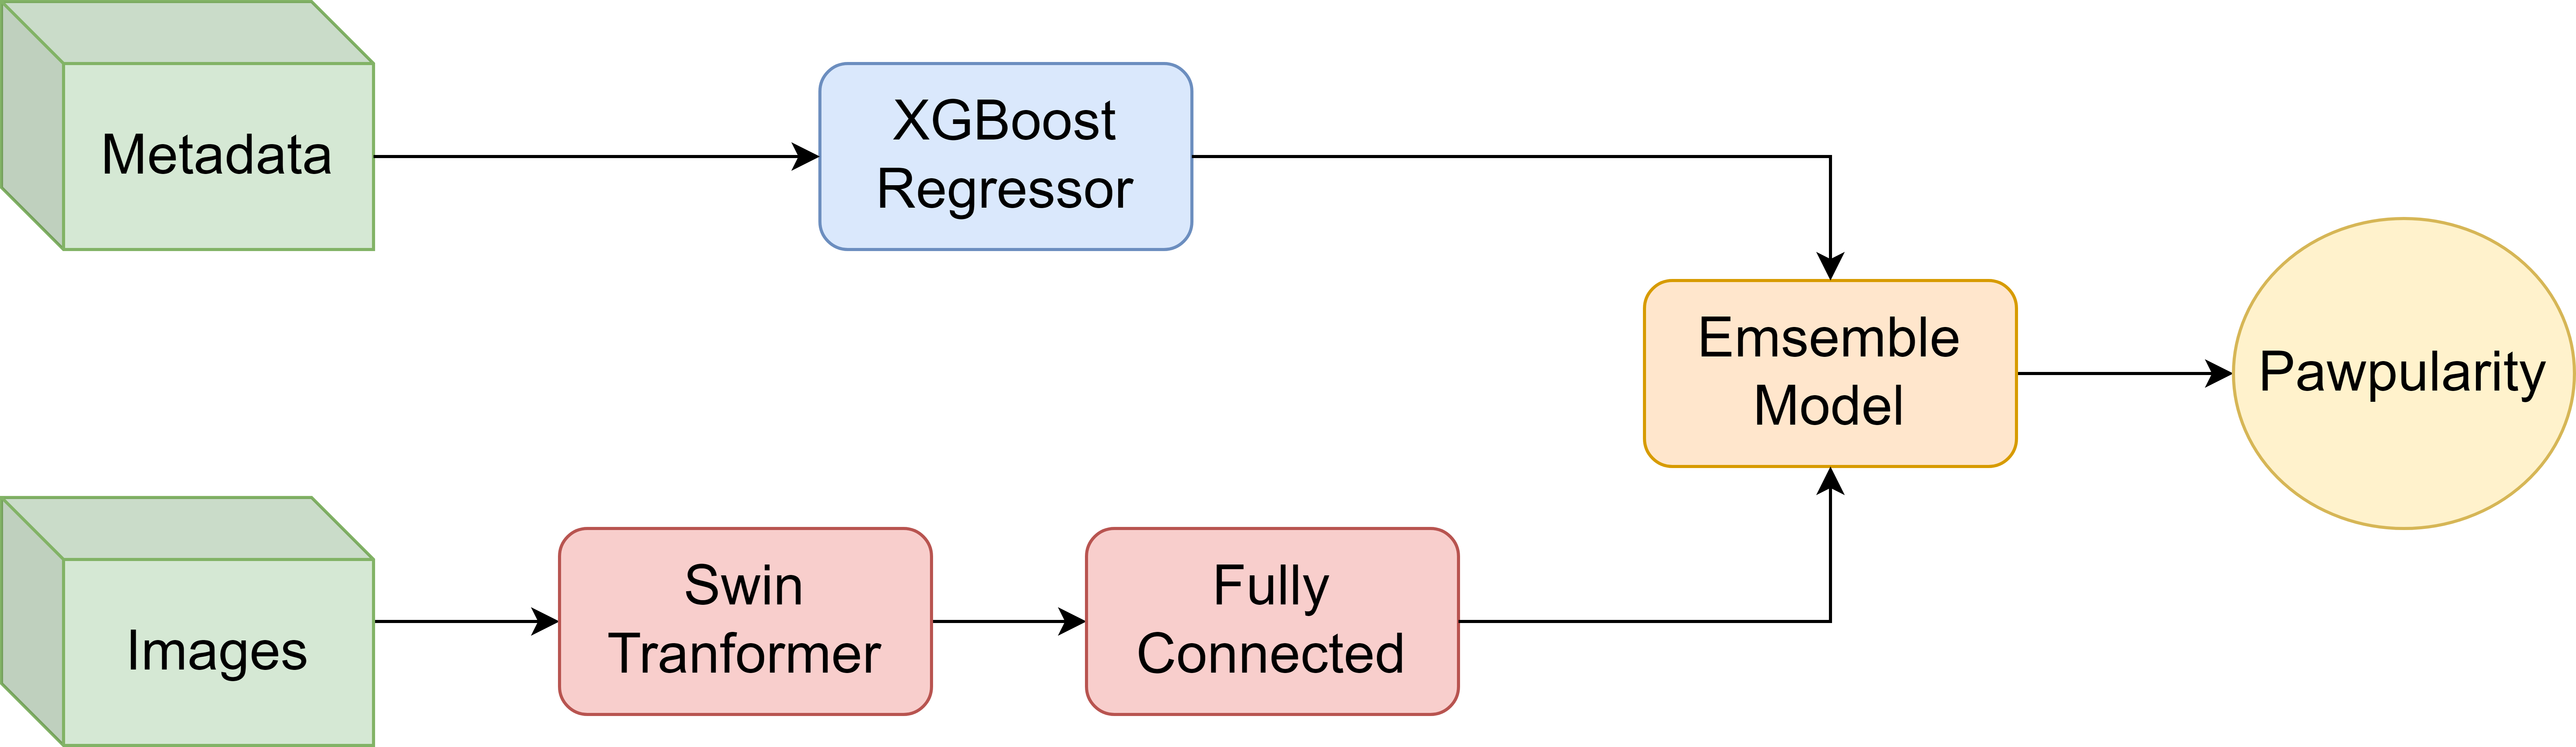
\includegraphics[width=0.8\linewidth]{figs/arch.png}
    \caption{Final solution architecture.}
    \label{fig:arch}
\end{figure}

As shown in the figure above, the Swin Transformer will be the backbone of our neural network, being responsible for feature extraction, which will be properly processed by the fully connected layer. In addition, we will also process the metadata features using an optimized distributed Gradient Boosting library for decision trees, XGBoost. Finally, after both models made their guesses, we use Optuna to maximize the respective Ensemble score on a validation set.

\subsubsection{Swin Transformer}
Fundamentally, our model will rely on a pretrained Swin Transformer as the backbone of our neural network, extracting valuable features which will be used by the fully connected layer. Over the pretrained model, we will train the model according the given dataset. Furthermore, we reframed the problem as a classification task instead of regression one, normalizing the target Pawpularity to [0, 1]. Therefore, we use Binary Cross Entropy Loss, which will better penalize worst predictions.

\begin{figure}[h!]
    \centering
    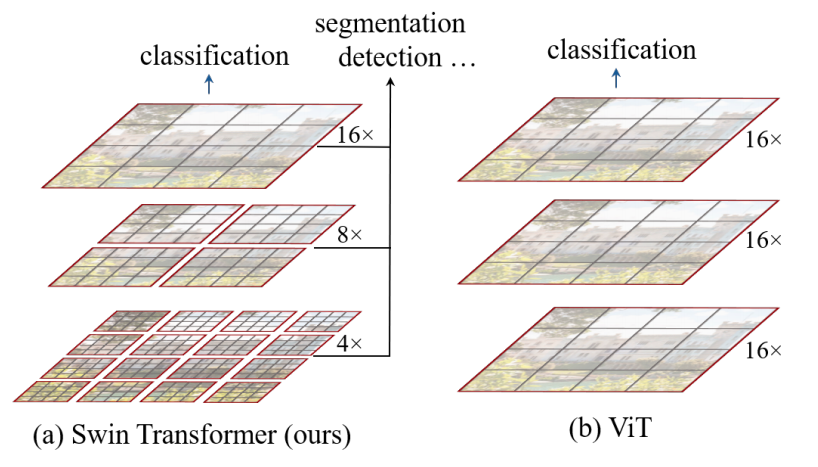
\includegraphics[width=0.7\linewidth]{figs/transformers.png}
    \caption{Swin and ViT approaches comparison.}
    \label{fig:transformers}
\end{figure}

The Swin Tranformer will calculate self-attention among images by ‘shifting windows’. The shifted windowing approach was what brought greater efficiency when compared with other transformers (Figure \ref{fig:transformers}). Finally, the complete Swin Transformer architecture is presented in Figure \ref{fig:swin}.

\vspace{1cm}

\begin{figure}[h!]
    \centering
    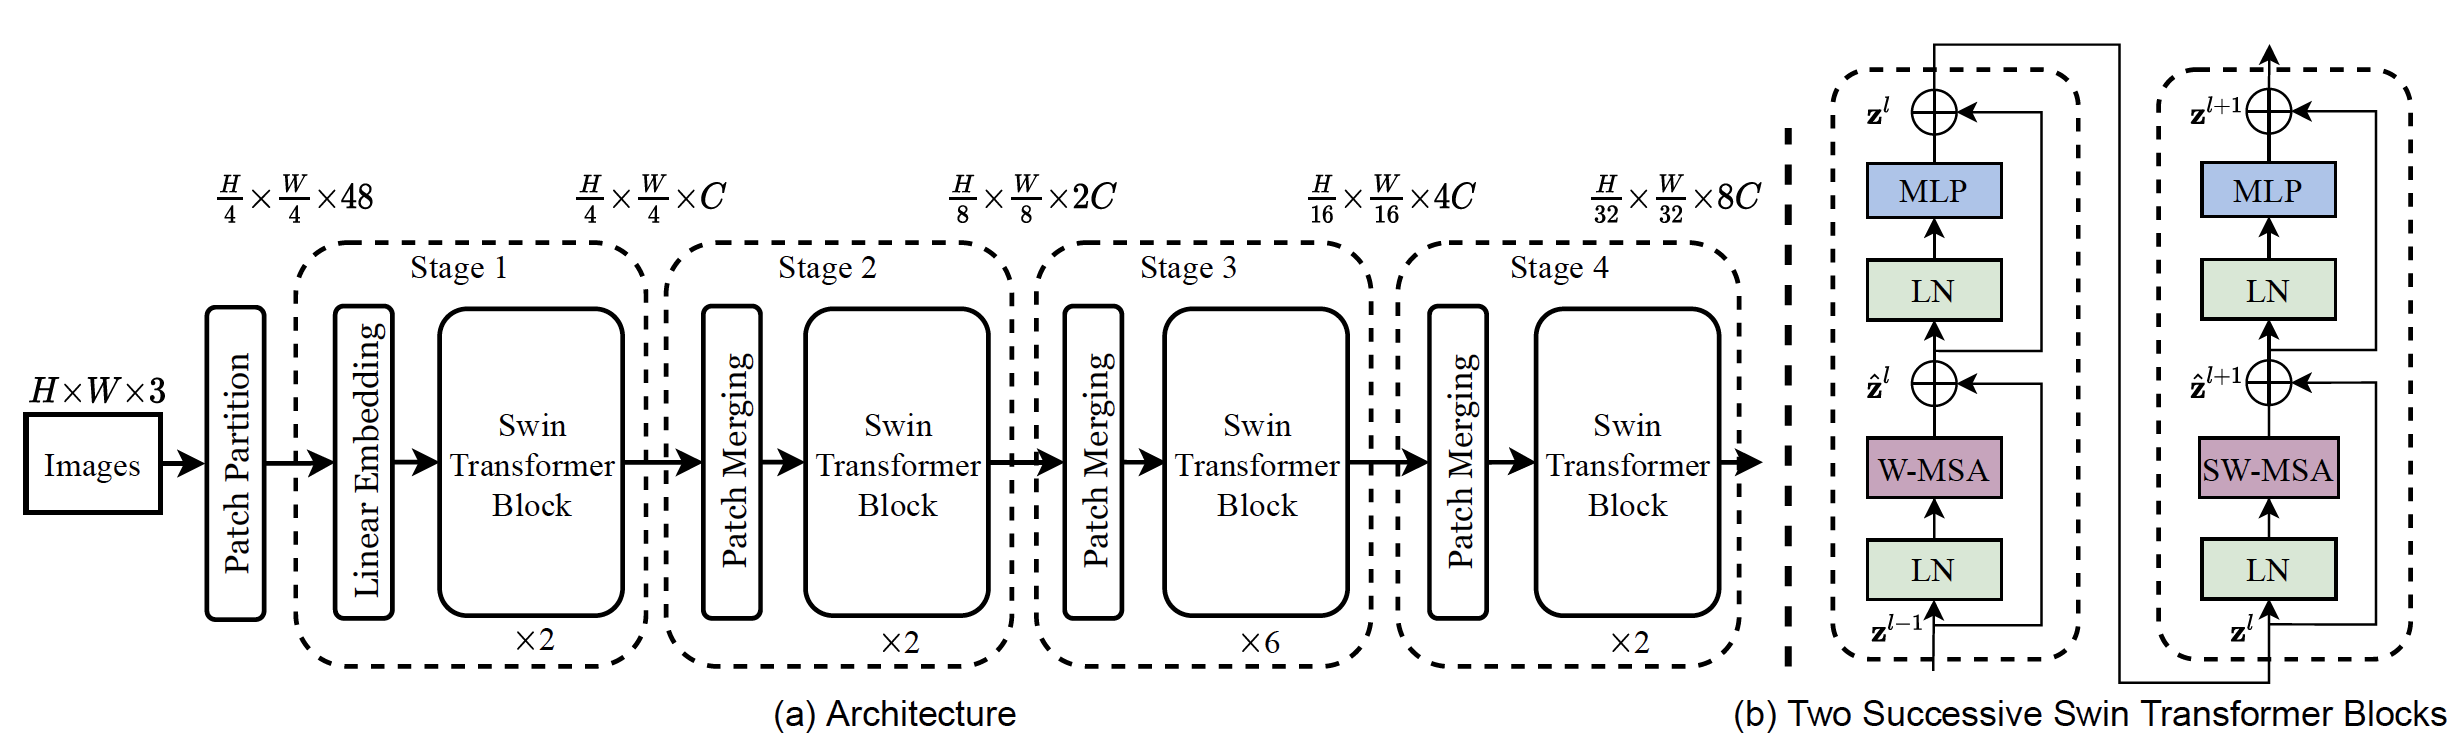
\includegraphics[width=1\linewidth]{figs/swin.png}
    \caption{Swin architecture.}
    \label{fig:swin}
\end{figure}

Moreover, a Stratified 10-Fold cross validation was implemented. In order to provide a uniform distribution, each strata will be fetched according percentiles. Finally, we will train the model for each fold, where the final Swin prediction will be the mean of every fold prediction. 


\subsubsection{XGBoost} \label{sec:xgb}
XGBoost tries to improve single weak models (in this case, decision trees) by combining them together, in order to generate a collectively strong model. Moreover, the addition of the generated weak models is formalized as a Gradient Descent algorithm, over an objective function. Each of the decision trees is added one at a time, and trained using the residual errors of their predecessors as labels, therefore, at each iteration, the focus is directed to the samples which have not yet been accurately predicted. XGBoost has been known to achieve impressive results, being the most used Gradient Boosting implementation for tabular data, regarding Kaggle competition winning solutions. Consequently, we decided integrate this model and see how it would perform on the given metadata features.\\
Similarly to the Swin Transformer, a Stratified 10-Fold cross validation was implemented and the final predictions resulted from calculating the mean of the ones from every fold.

\subsubsection{Ensemble Model using Optuna}
At first, we relied on the Swin Transformer to make our predictions in the competition using the pictures, and on XGBoost to make our predictions using the metadata features, individually. However, we decided to build an Emsemble Model which would take into account the predictions from both individual implementations, because, even though the Swin Transformer had the best performance so far, perhaps XGBoost was also extracting useful signals from the metadata that would complement the ones of Swin. Accordingly, we used Equation \ref{ensemble}, where we assign a weight to each model and calculate the corresponding weighted average for our predictions.\\
\begin{align} \label{ensemble}
    P = \sum_K w_k \cdot P_k\textrm{, \> where} \sum_K w_k = 1
\end{align}\\
We started by assigning weights according to the performance of each model during cross validation, so the Swin Transformer would have the largest weight. Afterwards, we decided to further tune the weights using Optuna, a fast AutoML framework which automates the trial-and-error procedure of optimizing hyper-parameters. Optuna uses a Bayesian Optimizer in order to intelligently focus the searching process in the ranges of values that present most potential. In the end, we were able to find an optimal combination and achieve improved results, which are presented in the following section.

\section{Experiments}
We have made a few submissions on \textit{Kaggle} for each of the implemented models. Their respective score was calculated using the Root Mean Squared Error (RMSE) between our predictions and the correct labels. The best results for each model may be found in Table \ref{tab:score}.\\
We have noticed in some of our testing that our model currently has a problem of high bias, resulting in  underfitting the data. As we investigated more about the problem and read public notebooks from the competition, we have concluded that the majority of the teams also is facing a similar situation. In fact, no mather how complex other team solutions could be, our best score is not that far from the best score in the competition, which is currently 17.50 (RMSE).\\
As shown on the scores table, both CNN and XGBoost models do not have outstanding results when compared to the baseline, where we predict the mean. Actually, these models will fail generalizing either to the train or test set. However, when the XGBoost model was ensembled with the pretrained Swin Transformer model, it slightly increased performance.

\begin{table}[h!]
\centering
\setlength{\extrarowheight}{3pt}
\begin{tabular}{|c|c|}
    \hline
    \textbf{Model} & \textbf{Public Score} (RMSE)\\
    \hline
    Baseline (Mean) & 20.59\\
    \hline
    CNN K-Fold & 20.56\\
    \hline
    XGBoost K-Fold & 20.49\\
    \hline
    Swin Transformer K-Fold & 18.04\\
    \hline
    \textbf{Swin Transformer K-Fold + XGBoost K-Fold} & \textbf{17.88}\\
    \hline
\end{tabular}
\vspace{0.3cm}
\caption{Different approaches and respective scores.}
\label{tab:score}
\end{table}

\section{Conclusion}
In conclusion, we started tackling this challenge as beginners in the field of Machine Learning. However, we were able to incrementally improve our solutions by performing thorough research on the topic and on the problem itself. Therefore, this project provided us an enriching learning experience, where we had the opportunity to apply the knowledge and techniques learned from the Machine Learning course, as well as from our own research, on a relevant real-work problem.\\
Regarding future work, we intend to further focus on the presented high bias situation, in order to conclude whether or not it is actually possible to extract more valuable signals from the given dataset, since it is extremely noisy.

\section{Work Contributions}
Both Armando and David started the project by implementing a first approach using a Convolutional Neural Network and K-Fold cross validation. Due to the poor scores of our initial model, we decided to tackle the different sides of the challenge in parallel, where Armando implemented a XGBoost model for the metadata, while David focused on integrating a Swin Tranformer model for the images, both using Stratified K-Fold with percentile distribution. Additionally, Armando designed an Ensemble model which would take into account both the Swin Transformer and the XGBoost predictions, using Optuna for optimal weight distribution. Both the elements worked together and cooperatively for the report.

\small
\printbibliography

\end{document}
